\chapter{Metodologia}\label{cap:metodologia}

Neste capítulo é descrita a sequência de etapas que serão realizadas neste trabalho para que os objetivos de pesquisa sejam alcançados.

Em imagens aéreas, como as utilizadas neste trabalho, é comum que os elementos que indicam presença humana sejam relativamente grandes (pista de pouso, estradas, clareiras, etc.), podendo ser definidas como uma região durante a segmentação da imagem. Portanto, classificar pixels tende a apresentar custo computacional elevado, visto que mesmo uma pequena imagem provê dezenas de milhares deles, que devem ter suas características extraídas e providas ao modelo de aprendizado, para que possam ser classificados. Portanto, utilizar técnicas de segmentação de imagem para agrupar os pixels espacialmente e caracteristicamente relacionados em uma única amostra não só possibilita uma execução mais rápida da solução computacional, como também torna o resultado final menos ruidoso.

Por este motivo, a arquitetura para a solução proposta neste trabalho prevê uma etapa de segmentação das imagens, seguida de uma etapa de classificação, responsável pela determinação do tipo de cada região encontrada na segmentação. Desta forma, elementos antrópicos podem ser separados como mais uma das regiões das imagens e classificados como tal. O diagrama da arquitetura geral da solução pode ser visto na figura \ref{fig:metDiagramaGeral}.

\begin{figure}[h]
    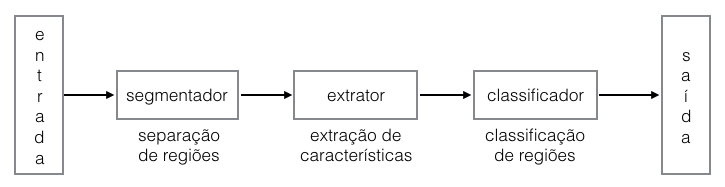
\includegraphics[width=\textwidth]{imgs/arquitetura_geral}
    \caption{Arquitetura geral da solução desenvolvida para detecção de elementos antrópicos em imagens aéreas da floresta amazônica.}
    \label{fig:metDiagramaGeral}
\end{figure}

A ideia geral é que imagens aéreas de regiões florestais da Amazônia legal sirvam de entrada para o problema. Estas mesmas imagens serão particionadas em regiões por um segmentador. Em seguida, um extrator será utilizado para criar o vetor de características de cada segmento provido pela etapa anterior. Por fim, um classificador composto por um ou mais algoritmos de classificação será utilizado para rotular as regiões, com a finalidade de encontrar as regiões de elementos antrópicos. A saída do sistema pode, então, ser composta pelas regiões segmentadas e suas classificações finais.

Embora esta seja uma arquitetura simples, bastante difundida na literatura, nuances para o problema apresentado neste trabalho devem ser levadas em conta. Para chegarmos à conclusão de quais segmentadores, extratores e classificadores devem ser utilizados, são necessárias várias etapas de experimentação, validação e análise de resultados.

\section{Entrada}

Uma base de dados com imagens aéreas de floresta tropical precisa ser formada. As imagens não precisam ter as mesmas dimensões, mas devem ter condições visuais claras do cenário e pertencerem à região de floresta amazônica, excluindo imagens de cidades e povoados da região.

Como serão processadas por uma etapa de segmentação, as imagens não sofrerão nenhum tipo de filtragem, ficando estas a cargo dos segmentadores a serem avaliados. A base de imagens gerada nesta etapa é um dos objetivos específicos deste trabalho.

\section{Segmentador}\label{sec:metSegmentador}

Para encontrarmos o segmentador ideal, os métodos de segmentação de imagens considerados estado-da-arte serão aplicados à uma parte da base de imagens aéreas da floresta amazônica. Conforme levantado no capítulo \ref{cap:trabalhos}, os seguintes métodos serão avaliados: Mean-shift, JSEG, MSEG, SRM, FSEG e gPb-owt-ucm. Estes métodos foram escolhidos por terem os melhores desempenhos no \textit{benchmark} de segmentação de uma base de imagens aéreas de \citeonline{yuan2:2013}.

Também será realizado um experimento que funde as etapas de segmentação e classificação em uma só, utilizando algoritmos de aprendizado de máquina supervisionados para segmentar as imagens diretamente para suas classes (floresta, água, etc) pixel a pixel. Isto é importante para determinar se há ganhos reais na separação entre segmentação e classificação das imagens, ou se realizar todo o procedimento em um único passo produz melhores resultados de acurácia e custo computacional.

A base de dados também precisa ser segmentada manualmente por seres humanos, pois este será o \textit{ground-truth} usado para aferir o desempenho dos algoritmos de segmentação avaliados. Ainda é preciso aferir a consistência da segmentação manual realizada por seres humanos. Métricas de erros de consistência como o \textit{Local Consistency Error} (LCE) e \textit{Global Consistency Error} (GCE), descritos na seção \ref{sec:avaliacaopdi}, devem ser aplicados para a medição de desempenho de todos os algoritmos, bem como para validação da consistência interna da segmentação manual.

Esta etapa deve determinar o método de segmentação com melhores resultados, a ser utilizado na solução descrita pelo trabalho. A precisão e o tempo de execução devem ser utilizados para a avaliação do desempenho dos algoritmos testados. Em seguida, é preciso extrair as características dos segmentos gerados.

\section{Extrator}\label{sec:metExtrator}

Os algoritmos de classificação lidam com variáveis numéricas inteiras, de ponto flutuante e em alguns casos, dados textuais. No entanto, para classificar imagens, ou no caso deste trabalho, segmentos de imagens, é preciso que um conjunto de características seja extraído dos pixels destas imagens ou regiões e disponibilizados para o modelo de classificação.

Nesta etapa serão testadas diversas características disponíveis na literatura de processamento digital de imagens, especialmente informações sobre cor, intensidade, textura e morfologia destas amostras. A escolha das características foi baseada, inicialmente, nas características utilizadas em trabalhos relacionados de classificação de imagens aéreas: canais RGB para descrição de cores, histogramas de intensidade, \textit{Local Binary Patterns} para descrição de texturas e transformada de Hough para detecção e descrição de formas geométricas, em especial linhas retas.

Os atributos também deverão passar por um processo de seleção baseada em correlação, o CFS. O objetivo é diminuir a dimensionalidade do vetor de características e avaliar se há ganho no desempenho e generalização dos algoritmos de aprendizado, utilizando este subconjunto do vetor de características original.

Como requisito da composição da base de dados de segmentos, bem como para avaliação e otimização do vetor de características, todas as amostras geradas pela etapa de segmentação devem ser rotuladas manualmente e contar com a avaliação de especialistas na inspeção deste tipo de imagem. Com a base devidamente criada e rotulada, experimentos para determinar os classificadores mais adequados podem ser feitos.

\section{Classificador}\label{sec:metClassificador}

Nesta etapa, quatro estratégias de classificação presentes na literatura serão abordadas: classificadores multi-classe, binários, unários e conjuntos de classificadores unários. Essas estratégias não demandam alterações na arquitetura geral da solução, mas mudam a forma como a base é rotulada e organizada. As métricas de avaliação do aprendizado precisam ser ponderadas para cada estratégia.

A motivação para explorar estas quatro abordagens é a diversidade de estratégias encontradas na literatura relacionada. É importante destacar que a classe de interesse, elementos antrópicos, permanece a mesma em todas as abordagens, e sua inspeção mais cuidadosa é vital na avaliação de todos os métodos utilizados. Como esta classe é absolutamente minoritária (<1\% das instâncias) na base de imagens utilizada no trabalho, abordagens que lidam com anomalias de forma mais robusta serão investigadas.

\subsection{Classificador multi-classe}

Nesta estratégia, a base de segmentos gerada será rotulada entre cinco classes possíveis: floresta, vegetação rasteira, água, terra e elemento antrópico. A escolha das classes foi feita através de uma observação das classes de trabalhos relacionados.

Também observando os algoritmos utilizados em trabalhos relacionados que modelam o problema como uma questão multi-classe, diversos métodos de classificação multi-classe serão testados: \textit{Random Forest}, KNN, SVM, árvore de decisão e \textit{Naive Bayes}. Esta gama de métodos também serve para cobrir os testes com abordagens de aprendizado simbólico, bayesiano, aprendizagem preguiçosa (do inglês \textit{lazy learning}) e ensemble de classificadores multi-classe.

Todos os métodos devem ser testados com a base completa de segmentos, mas também com a base pré-processada por um seletor de características, que será responsável pela redução do vetor de características do problema. Este detalhe do experimento servirá para determinar se a seleção de atributos nesta abordagem reduz a complexidade dos modelos gerados e o ruído na base de dados, possibilitando melhor taxa de aprendizagem.

Cada algoritmo deve ser responsável pela classificação de toda a base. Ao fim, métricas de aprendizado como acurácia, precisão e revocação serão utilizadas para comparar os métodos entre si.

\subsection{Classificador binário}

Neste cenário, a base de segmentos gerada será rotulada entre duas classes: elementos naturais e elementos antrópicos. A classe de elementos naturais agrupa o que originalmente seriam as classes de floresta, vegetação rasteira, água e terra. A motivação desta modelagem é realizar experimentos com algoritmos que permitam o aprendizado bi-classe, abordagem pouco usada nos trabalhos encontrados na literatura, bem como avaliar se o agrupamento das classes secundárias (as classes que não são de elementos antrópicos), pode ser descrito de forma eficaz pelos algoritmos testados.

Os classificadores utilizados serão os mesmos do experimento com classificadores multi-classe, visto que não há grande diferença metodológica nas duas abordagens. Todos os métodos também serão testados com seletores de características, e o impacto desta seleção também será avaliado.

Ao fim do experimento, as métricas propostas para o problema de aprendizado serão colhidas para cada método testado, e utilizadas para comparar os métodos entre si.

\subsection{Classificador unário}

Assim como no experimento de classificadores binários, a base de dados de segmentos será dividida entre elementos naturais e elementos antrópicos, utilizando os mesmos critérios. À primeira vista, esta estratégia de aprendizado parece muito similar aos classificadores binários, mas a diferença está inicialmente nos algoritmos utilizados.

Os métodos de classificação unária tendem a lidar melhor com bases de dados cujas classes estão fortemente desbalanceadas, provável caso da base de imagens utilizada neste trabalho, especialmente depois do rearranjo entre elementos antrópicos e demais classes de elementos naturais. Por esta razão, a abordagem que utiliza classificadores unários precisa ser avaliada.

Como o aprendizado unário utiliza o conceito de classe majoritária e classe anômala (\textit{outlier}), é preciso definir quais classes do problema exercerão estes papéis. Por uma simples questão de frequência estatística, fica definido que a classe de elementos naturais é a classe majoritária, enquanto a classe de elementos antrópicos é considerada a classe anômala.

Apoiando-se nos casos apresentados pela literatura, em especial nos trabalhos relacionados que se propõem a realizar detecção de anomalias, os algoritmos utilizados neste experimento serão os \textit{One-Class Support Vector Machines} (OC-SVM) e o REPTree. Aqui também deve ser avaliado o impacto de um seletor de atributos aplicado ao vetor de características da base de dados, a fim de entender se há mudança significativa na taxa de aprendizado da classe anômala.

\subsection{Conjunto de classificadores unários}

Esta abordagem consiste na criação de modelos de aprendizado unários para cada classe do problema, exceto para a classe anômala, e posteriormente na combinação dos resultados destes classificadores unários para um resultado multi-classe. Sendo assim, um ou mais classificadores unários serão treinados para cada uma das classes de floresta, vegetação rasteira, água e terra. A motivação por trás do uso desta abordagem é o crescente número de trabalhos na literatura de classificação de imagens que utiliza este grupo de técnicas, em especial trabalhos que discorrem sobre descrição de objetos em grandes coleções de imagens.

A preparação da base de dados é um importante passo nesta estratégia de aprendizado, visto que diversas versões da base de segmentos terão de ser geradas, cada uma representando a classe não-anômala em questão como a classe majoritária e todas as demais como anomalias.

O classificadores criados serão agrupados em um \textit{ensemble} de classificadores e cada um dos modelos será utilizado na composição do veredito final, para a classificação da amostra. Por uma limitação de escopo do trabalho, uma abordagem simples de votação com pesos deve ser utilizada. Os pesos utilizados, bem como as implicações desta abordagem devem ser discutidas nos resultados do experimento.

Assim como todas as outras estratégias de classificação presentes neste trabalho, as métricas mais relevantes serão a acurácia, precisão e revocação da classe de interesse, de elementos antrópicos, que aqui é a classe anômala. As abordagens de classificação com melhor desempenho nestes quesitos ou mais promissoras devem ser apontadas ao fim destes experimentos.

\section{Saída}

 Os resultados dos experimentos anteriores devem sustentar a conclusão sobre quais métodos de segmentação e classificação são mais indicados para a solução. A saída da solução deve indicar quais segmentos da coleção de imagens original possuem elementos antrópicos. A avaliação do desempenho na detecção destes elementos é a métrica definitiva da adequação da solução para o problema proposto.

O próximo capítulo descreve os experimentos realizados e discute os resultados encontrados.